
\chapter{Optical Fiber Impairments}
\label{chap:fiber_impairments}


\section{Introduction}

Propagation through an optical fiber distorts a frequency signal. Previous work described the various optical impairments in an optical fiber and their influence on a frequency signal \cite{menyukIFCS2015}. In this chapter, we summarize that work and relate it to our simulations.

The optical fiber communication system transmits information over multiple data signals separated in the frequency domain in a scheme called Wavelength Division Multiplexing (WDM). The data signals have center frequencies that are spaced $10$--$100$ GHz apart and are on the order of $100$ THz in agreement with the ITU standard \cite{ITU-T2012}. A frequency signal will have a smaller bandwidth than the data signals and can be included alongside the data traffic. The frequency signal's bandwidth is also small enough that we can place the frequency signal between two data signals that are centered at adjacent center frequencies as shown in Figure~\ref{fig:system}. However, placing the frequency signal in this manner increases the nonlinear coupling between the neighboring data signals and the frequency signal and thus increases the distortion of the frequency signal.

\begin{figure}
	\centering
	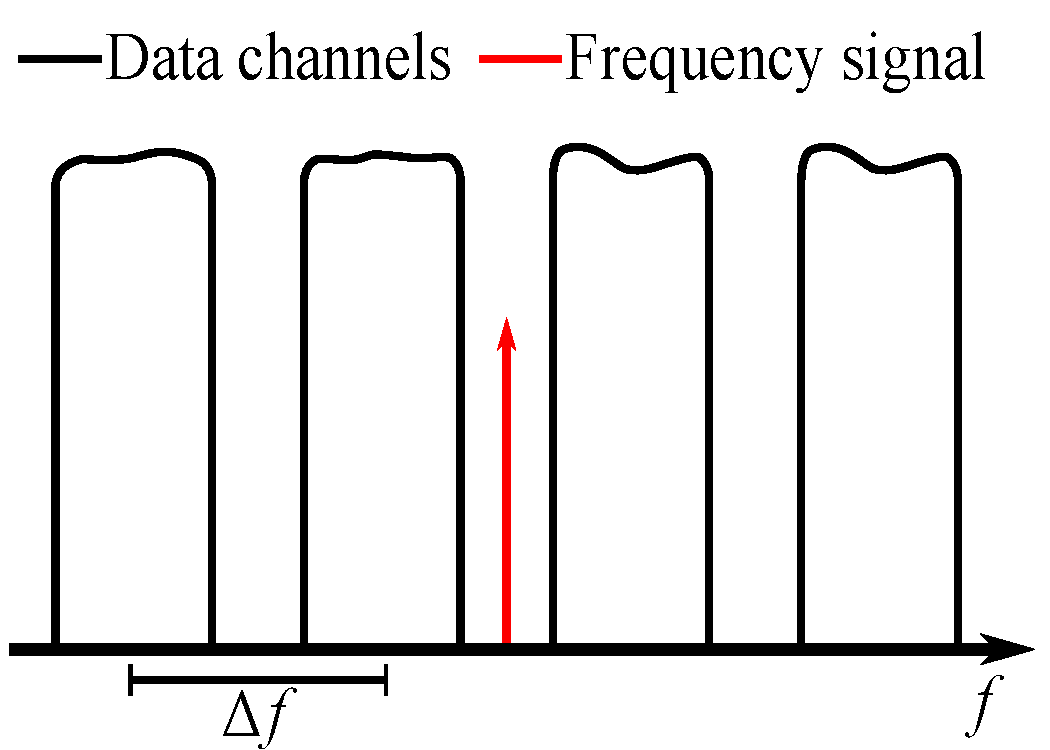
\includegraphics[scale=0.6]{img/system.pdf}
	\caption{Desired frequency domain placement of the frequency signal}	\label{fig:system}
\end{figure}

We assume an optical fiber communication system with multiple data signals in a WDM setup around the wavelength $1530$ nm with a bandwidth of $10$ GHz. The data signals are modulated as non-return to zero on-off-keyed (NRZ-OOK) symbols. The fiber is considered a single mode fiber with second-order dispersion, Kerr nonlinearity, and attenuation constant in the frequency range of application.

In this chapter we first examine coupled propagation equations for a single data signal and frequency signal separated in the frequency domain. Then we generalize the coupled equations for multiple data signals and a single frequency signal. These equations include common optical impairments in a commerical optical fiber communication system. We further examine each of the impairment terms in the equations, and we will give suitable conditions under which they can be neglected when calculating the phase stability. We will then show that the impairment known as cross-phase modulation is the primary optical source of phase instability.

\section{Coupled Propagation Equations} \label{sec:cnlse}

The small bandwidth compared to the center frequency allows us to use a slowly varying envelope approximation to the propagation of the signals in the optical fiber. The electric field becomes a sum of the products of a rapidly varying carrier signal and a slowly varying envelope,
%
\begin{equation}
\mathbf{E}(\mathbf{r}, t) = \frac{1}{2}\hat{x}\left[ E_1\exp(-i\omega_1t) + E_2\exp(-i\omega_2t)\right] + c.c.,
\end{equation}
%
where $\hat{x}$ is the direction of polarization, $\omega_j$ for $j=1,2$ are the carrier frequencies for the two signals, and $E_j$ are the slowly varying time envelopes of the two signals. We assume each of the envelopes may be separated into the form,
%
\begin{equation}
E_j(\mathbf{r}, t) = F_j(x,y)u_j(z,t)\exp(i\beta_{0j}z),
\end{equation}
%
where $j=1,2$ corresponding to the appropriate envelope, $F_j(x,y)$ is the distribution of the fiber mode in the plane normal to the propagation direction for the $j$th field, $u_j(z,t,)$ is the slowly varying amplitude, and $\beta_{0j}$ is the phase shift associated with propagation distance. We then get a solution for the envelope $u_j$ in the form of the nonlinear Schr{\"o}dinger (NLS) equation,
%
\begin{equation}
\frac{\partial u_j}{\partial z} + \beta_{1j}\frac{\partial u_j}{\partial t} + \frac{i\beta_{2j}}{2}\frac{\partial^2 u_j}{\partial t^2} + \frac{\alpha_j}{2}u_j = \frac{in_2\omega_j}{c}\left(f_{jj}|u_j|^2 + 2f_{jk}|u_k|^2\right)u_j,
\end{equation}
%
where $j\neq k$, $j,k = 1,2$ for the two signals, $\beta_{1j} = 1/v_{gj}$ is the inverse group velocity of the corresponding signal, $\beta_{2j}$ is the group velocity dispersion of the corresponding signal, and $\alpha_j$ is the attenuation. The terms on the right-hand side represent the nonlinear impairment, $n_2$ is the nonlinear Kerr parameter and the $f_{jk}$ are the overlap integrals defined by $F_j$,
%
\begin{equation}
f_{jk} = \frac{\int_{-\infty}^{\infty}\int_{-\infty}^{\infty} |F_j(x,y)|^2|F_k(x,y)|^2dxdy }{\int_{-\infty}^{\infty}\int_{-\infty}^{\infty} |F_j(x,y)|^2dxdy\int_{-\infty}^{\infty}\int_{-\infty}^{\infty}|F_k(x,y)|^2dxdy}
\end{equation}
%
Since the system has conventional single mode fibers, the overlap integrals $f_{jk}$ have a small difference. We neglect that difference and write the integrals as $f_{11} = f_{12} = f_{22} = 1/A_{\text{eff}}$. This allows us to simplify the right-hand side further by introducing the nonlinear parameter $\gamma = (n_2\omega_j)/(cA_{\text{eff}})$. Though the $\omega_j$ and $A_{\text{eff}}$ have frequency dependence, $\gamma$ remains fairly constant around the $1.5$ $\mu$m wavelength range for conventional single-mode fibers.

We replace the subscript $j=1,2$ with $j=d,f$ where the $d$ refers to the data signal and the $f$ refers to the frequency signal. Then the two coupled equations become
%
\begin{subequations}
\begin{align}
\frac{\partial u_d}{\partial z} + \beta_{1d}\frac{\partial u_d}{\partial t} + \frac{i\beta_{2}}{2}\frac{\partial^2 u_d}{\partial t^2} + \frac{\alpha}{2}u_d &= i\gamma\left(|u_d|^2 + 2|u_f|^2\right)u_d, \label{eq:cdprop} \\
\frac{\partial u_f}{\partial z} + \beta_{1f}\frac{\partial u_f}{\partial t} + \frac{i\beta_{2}}{2}\frac{\partial^2 u_f}{\partial t^2} + \frac{\alpha}{2}u_f &= i\gamma\left(|u_f|^2 + 2|u_d|^2\right)u_f. \label{eq:cfprop}
\end{align}
\end{subequations}
%
It is extremely useful to transform into the retarded time with respect to the frequency signal, $T = t - \beta_{1f}z$, $z' = z$. Then we use the chain rule to get
%
\begin{subequations}
\begin{align}
\frac{\partial u_j}{\partial z} &= \frac{\partial u_j}{\partial z'}\frac{\partial z'}{\partial z} + \frac{\partial u_j}{\partial T}\frac{\partial T}{\partial z} =  \frac{\partial u_j}{\partial z'} - \beta_{1f}\frac{\partial u_j}{\partial T}, \\
\frac{\partial u_j}{\partial t} &= \frac{\partial u_j}{\partial z'}\frac{\partial z'}{\partial t} + \frac{\partial u_j}{\partial T}\frac{\partial T}{\partial t} =  \frac{\partial u_j}{\partial T}, \\
\frac{\partial^2 u_j}{\partial t^2} &= \frac{\partial^2 u_j}{\partial T^2}.
\end{align}
\end{subequations}
%
This will cancel out the term with $\beta_{1f}$ in Eq.~\ref{eq:cfprop} and the corresponding term in Eq.~\ref{eq:cdprop} becomes a difference between the two, $\delta = \beta_{1d} - \beta_{1f} = (v_{gf} - v_{gd})/(v_{gf}v_{gd})$,
%
\begin{subequations}
\begin{align}
\frac{\partial u_d}{\partial z'} + \delta\frac{\partial u_d}{\partial T} + \frac{i\beta_{2}}{2}\frac{\partial^2 u_d}{\partial T^2} + \frac{\alpha}{2}u_d &= i\gamma\left(|u_d|^2 + 2|u_f|^2\right)u_d, \label{eq:dataprop} \\
\frac{\partial u_f}{\partial z'} + \frac{i\beta_{2}}{2}\frac{\partial^2 u_f}{\partial T^2} + \frac{\alpha}{2}u_f &= i\gamma\left(|u_f|^2 + 2|u_d|^2\right)u_f. \label{eq:freqprop}
\end{align}
\end{subequations}
%

The two terms that are dependent on the optical powers of the signals in the propagation equations represent two different forms of nonlinear phenomenon of the fiber, self-phase modulation and cross-phase modulation. There is another nonlinear phenomenon that appears as noise at center frequencies that are a linear combination of the signals' center frequencies known as four-wave mixing. When restricted to two signals, it is not possible for four-wave mixing to occur with a center frequency equal to either of the signals'. However, four-wave mixing is capable of producing something at the frequency signal's carrier frequency in a system with more data signals.

\section{Multiple Data Channels} \label{sec:multiple}

The previous section showed how two copropagating signals can nonlinearly couple creating parasitic signals and inducing a phase shift on each other. Multiple data signals will also couple with the frequency signal and their fellow data signals. This means that every data signal in the system can contribute a phase shift in the frequency signal. Supposing there are $n$ data signals at center frequencies $\omega_k$, there now becomes a set of $n+1$ propagation equations
%
\begin{subequations}
\begin{align}
\frac{\partial u_{dk}}{\partial z'} + \delta_k\frac{\partial u_{dk}}{\partial T} + \frac{i\beta_{2}}{2}\frac{\partial^2 u_{dk}}{\partial T^2} + \frac{\alpha}{2}u_{dk} &= i\gamma\left(|u_{dk}|^2 + 2|u_f|^2 + 2\sum_{\substack{m=1\\ m\neq k}}^n|u_{dm}|^2\right)u_{dk}, \label{eq:mdataprop} \\
\frac{\partial u_f}{\partial z'} + \frac{i\beta_{2}}{2}\frac{\partial^2 u_f}{\partial T^2} + \frac{\alpha}{2}u_f &= i\gamma\left(|u_f|^2 + 2\sum_{m=1}^n|u_{dm}|^2\right)u_f. \label{eq:mfreqprop}
\end{align}
\end{subequations}
%
where the subscript $k,m$ in the data envelopes refers to the $k$th or $m$th data signal, the $\delta_k$ refers to the difference $\beta_{1k} - \beta_{1f}$ based on the different group velocities of the signals. The parameters $\beta_2$, $\alpha$, and $\gamma$ can be treated as constant over the limited frequency range of our signals.

Four-wave mixing now becomes a concern if $\omega_k + \omega_m = 2\omega_f$ and will appear in the frequency signal if they also satisfy the phase-matching condition $\beta(\omega_k) + \beta(\omega_m) = 2\beta(\omega_f)$. If those two conditions are satisfied, then Eq.~\ref{eq:mfreqprop} includes the four-wave mixing term, $2\gamma u_f^*u_mu_n$.

We are now prepared to summarize the optical impairments found in the propagation equations \ref{eq:mdataprop} and \ref{eq:mfreqprop}. These impairments are typical in commercial optical fiber communication systems and are limited and compensated for reliable data communication. However, frequency signals need accuracy, so we primarily explain the impact of the impairments on the frequency signal and give limitations to reduce their effects.

\section{Optical Impairments} \label{sec:impair}

In the previous sections, we showed how the nonlinear term creates multiple nonlinear terms. In this section, we describe how each of the terms relates to an optical impairment and how that impairment affects the frequency signal. In the analysis, we discuss conditions under which many of the optical impairments become negligible.

\subsection{Attenuation and Amplified Spontaneous Emission (ASE) Noise}
%
Attenuation appears in the decoupled equations above as
%
\begin{equation}
\diffp{u_f}{z} = -\frac{\alpha}{2}u_f.
\end{equation}
%
The attenuation is due to absorption and scattering and will lead to an exponential decrease of the optical power. Amplifiers are spaced periodically to compensate for the loss of optical power, but they add amplified spontaneous emisssion (ASE) noise. ASE noise is accurately described over the bandwidth of an optical signal as a white noise source with noise power \cite{agrawal2012fiber}
%
\begin{equation}
\sigma^2_{ASE} = n_{sp}h\nu_0 (G-1)\Delta\nu,
\end{equation}
%
where $n_{sp}$ is called the spontaneous emission factor, $h$ is Planck's constant, $\nu_0$ is the center frequency, $G$ is the gain of the amplifier, and $\Delta\nu$ is the bandwidth of the signal. 

Consider an optical communication system that has a distance of $800$ km and an $80$-km amplifier separation operating at the wavelength $1.5$ $\mu$m with loss $\alpha_{\text{dB}} = 0.2$ dB/km, which implies a gain $G=40$. A typically amplifier will have a noise figure $n_{\text{sp}} = 2$ with a total of $10$ amplifiers. If we suppose that the narrow bandwidth of the frequency signal is on the order of $10$ MHz, then the total noise power is $1$ nW. If the frequency signal has a power of $1$ $\mu$W or above, the effect of the noise on the frequency signal will be negligible, while its power is small compared to the power in a data signal, which is typically on the order of $1$ mW. Hence, it is possible to simultaneously make the impact of ASE noise on the frequency signal negligible, while ensuring that it does not nonlinearly affect the data signals.

\subsection{Chromatic Dispersion}

The dispersion appears as
%
\begin{equation}
\diffp{u_f}{z} = -\frac{i\beta_{2}}{2}\diffp{^2u_f}{T^2}.
\end{equation}
%
This impairment leads to pulse spreading of the optical signal because its frequency components travel at different velocities. The time spread due to dispersion is \cite{agrawal2012fiber}
%
\begin{equation}
\tau_{\text{disp}} = -\frac{2\pi c}{\lambda^2}\beta_{2f} L\Delta \lambda 
\end{equation}
%
where $L$ is the length of the fiber, and $\Delta\lambda$ is the range of wavelengths. For the optical communication system in the previous example and the frequency signal centered at a wavelength $\lambda \approx 1.5$ $\mu$m, we find $\tau_{\text{disp}} = 1$ ps. By contrast, the time slot of a single bit at $10$ Gbps occupies $100$ ps; so, dispersion can be neglected for the frequency signal. In this respect, the frequency signal differs significantly from a data signal, which typically has a bandwidth on the order of $10$ GHz.


%\subsection{Scattering}
%
%Scattering doesn't have explicit terms in the decoupled equations above. They will affect the signals in the form of attenuation and the creation of parasitic waves. We split up the types of scattering into those two cases:
%
%\subsubsection{Rayleigh Scattering}
%
%During fiber fabrication, the crystal lattice can form nonuniformly and create density variations along its length. This form of scattering contributes to the majority of loss and is covered above.
%
%\subsubsection{Brillouin and Raman Scattering}
%
%Optical waves can couple with acoustic waves and form optical waves of a lower frequency. These parasitic waves sap energy from the frequency signal.


\subsection{Self-Phase Modulation (SPM)}

The term
\begin{equation}
\diffp{u_f}{z} = i\gamma|u_f|^2u_f
\end{equation}
corresponds to self-phase modulation. This distortion takes the form of a phase shift dependent on the signal power. Thus, linear attenuation limits the effect over some length after each amplifier. The effective length is $L_{\text{eff}} = (1/\alpha)[1-\exp(-\alpha L)]$, so that $L_{\text{eff}} \approx 20$ km for $\alpha_{\text{dB}} = 0.2$ dB/km.

The maximum phase shift due to self-phase modulation for a length of fiber between amplifiers is \cite{Agrawal2013}
%
\begin{equation} \label{eq:maxspm}
\phi_{\text{SPM}} = \gamma P_f L_{\text{eff}},
\end{equation}
%
where $P_f$ is the power of the frequency signal. The total maximum phase shift is Eq.~\ref{eq:maxspm} multiplied by the number of amplifiers in the fiber link. For our system, $\gamma = 1.3$ W$^{-1}$km$^{-1}$, $L_{\text{eff}} = 20$ km, and $10$ amplifiers. If we impose an upperbound on $\phi_{\text{SPM}}$ of 1 radian, then the upper bound on the frequency signal power is $3.8$ mW.

\subsection{Four-Wave Mixing (FWM)}

The term
%
\begin{equation}
i\gamma u_f^*u_{dm}u_{dn}
\end{equation}
%
corresponds to four-wave mixing. For any two data signals centered at $\omega_m$ and $\omega_n$ with corresponding wavenumbers $\beta(\omega_m)$ and $\beta(\omega_n)$, four-wave mixing (FWM) creates a parasitic wave whenever $\omega_m + \omega_n = 2\omega_f$ and $\beta(\omega_m) + \beta(\omega_n) = 2\beta(\omega_f)$. This phase-matching condition is avoidable as long as the signals are located away from the zero-dispersion wavelength of the fiber. Placing the frequency signal greater than five times its bandwidth away from the zero-dispersion wavelength will eliminate this impairment \cite{menyukIFCS2015}.

\subsection{Cross-Phase Modulation (XPM)}

The remaining term,
\begin{equation}
\diffp{u_f}{z} = i2\gamma|u_d|^2u_f
\end{equation}
corresponds to cross-phase modulation (XPM), which leads to cross-talk between two signals. This effect becomes negligible when the group velocity difference between the data signal and frequency signal is large, which occurs when the two signals are spaced far apart in the frequency spectrum. Therefore, the effects of XPM on the frequency signal only has to be computed for the two neighboring data signals. Since our goal is to place the frequency signal between two data signals, XPM is the primary source of frequency distortion. The limitation on the optical power of the frequency signal ($\ll 1$ mW) implies that the effect of XPM due to the frequency signal on the data signals can be neglected.

\section{Phase noise on the frequency signal} \label{sec:noisexpm}

The data signals will be random strings of bits. We simplify the problem by using pseudorandom binary strings for our data signal \cite{PRBS}. Randomness also restricts our analysis to the impact on the frequency signal in the mean. The average behavior of the two neighboring data signals on the frequency signal can be considered equal. We simplify the effect of XPM on the frequency signal by replacing the two neighboring data signals influence with a doubling of a single data signal.

Then, applying the limits on the system parameters that we have obtained, Eqs. \ref{eq:mdataprop} and \ref{eq:mfreqprop} simplify to the following equations,
%
\begin{subequations}
\begin{align}
\label{eq:simpledfreq}
&\diffp{u_f}{z} = i4\gamma|u_d|^2u_f, \\
\label{eq:simpleddata}
&\diffp{u_d}{z} + \delta\diffp{u_d}{T} + \frac{i\beta_{2}}{2}\diffp{^2u_d}{T^2} + \frac{\alpha}{2}u_d = i\gamma|u_d|^2u_d.
\end{align}
\end{subequations}
%
The dispersion, SPM, FWM, and attenuation are considered negligible for the frequency signal. The non-neighboring data signals have enough frequency separation from the frequency signal to treat their contribution to the XPM negligibly. The effect of XPM has been doubled to represent the mean behavior of the two neighboring data signals. A low optical power of the frequency signal makes the effect of XPM on the data signal from the frequency signal to be negligible, and the data signals are separated enough to limit their contributions to the XPM on each other. 

The frequency signal has the form $u_f(z,T) = u_f(0,T)\exp[i\phi(z,T)]$, where $u_f(0,T)$ is the initial frequency source and $\phi(z,T)$ is phase distortion due to XPM. We may integrate Eq.~\ref{eq:simpledfreq}, from which it follows that
%
\begin{equation} \label{eq:phasedistort}
	\phi(z',T) = 4\gamma\int_0^{z'} |u_d(\zeta, T)|^2 d\zeta.
\end{equation}
%
The data signal is subject to the effects of loss, dispersion, a time shift due to the group velocity difference from the frequency signal, and self-phase modulation. The phase distortion of the frequency signal depends entirely on the evolution of the data signal as it propagates through the fiber.

\section{Chapter Remarks} \label{sec:3conc}

By limiting the frequency signal's optical power and its bandwidth, we can limit the causes of phase distortion due to optical impairments. As a consequence, the distortion will be dominantly due to XPM. In the next chapter, we perform computations to estimate $\phi(z,T)$ using typical system parameters for a commercial optical fiber communication system.